\chapter{Tecnologie di localizzazione}

Le tecnologie di localizzazione sono delle combinazioni di metodi e tecniche 
per determinare la posizione fisica di un oggetto o persona nel mondo reale.

Ci sono varie tecniche che differiscono per precisione (accuracy),
costo, modalità di disposizione (deployment), pervasività.

Un sistema di localizzazione è composto da due parti principali:

\begin{itemize}
\item
  \begin{quote}
  un set di nodi che possono trovarsi in stati diversi: \textbf{unknown}
  (posizione non nota), \textbf{settled} (posizione nota ma tramite
  inferenza) e \textbf{beacon} (landmark, posizione nota a priori)
  \end{quote}
\item
  \begin{quote}
  un algoritmo, da utilizzare per inferire o calcolare la posizione dei
  nodi sconosciuti.
  \end{quote}
\end{itemize}

Fortunatamente il GPS non è l'unica alternativa per la localizzazione,
perché è costoso e consuma tanta energia (l'antenna deve essere sempre
attiva) e deve esserci una comunicazione diretta con il satellite (non
funziona in-door).

Altri meccanismi di localizzazione si basano su proprietà fisiche delle
onde (\textbf{Received Signal Strength RSSI}, \textbf{Time of Arriva
ToA}). oppure sulla comunicazione wireless, ad esempio per demandare ad
un nodo più potente il calcolo della posizione.

Tra le varie applicazione della localizzazione possiamo trovare:

\begin{itemize}
\item
  \begin{quote}
  resource tracking
  \end{quote}
\item
  \begin{quote}
  finding someone or something (healtcare)
  \end{quote}
\item
  \begin{quote}
  proximity based service (notification or actuation, advertisement)
  \end{quote}
\end{itemize}

\subsection[Tassonomia delle tecniche di
localizzazione]{\texorpdfstring{Tassonomia delle tecniche di
localizzazione
\protect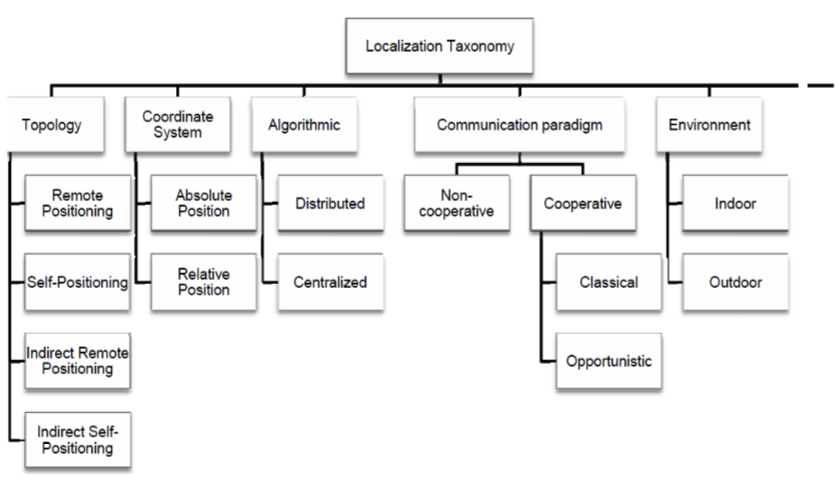
\includegraphics[width=6.26772in,height=3.68056in]{image5b.png}}
{Tassonomia delle tecniche di localizzazione}}
\label{tassonomia-delle-tecniche-di-localizzazione}

\begin{itemize}
\item
  \begin{quote}
  \textbf{Topology:} dove viene determinata la posizione del nodo, se in
  locale o tramite un'unità centrale. Come viene misurata l'intensità
  del segnale, se dal nodo oppure se viene comunicata da un ancora:
  \end{quote}

  \begin{itemize}
  \item
    \begin{quote}
    \textbf{Remote positioning:} una stazione centrale determina la
    posizione dei nodi tenendo conto dell'intensità del segnale ricevuto
    da vari nodi ancora. Il trasmettitore (nodo) è mobile e le unità
    ancora sono fisse in locazioni conosciute. (tracking degli animali
    in un parco)
    \end{quote}
  \item
    \begin{quote}
    \textbf{Self positioning}: il nodo stabilisce la sua posizione
    tenendo conto dell'intensità del segnale ricevuto dai vari nodi
    ancora. I nodi ancora sono in posizioni fisse e note (GPS)
    \end{quote}
  \item
    \begin{quote}
    \textbf{Indirect remote positioning}: il nodo determina con
    \textbf{self positioning} la sua posizione e la invia ad una
    stazione centrale.
    \end{quote}
  \item
    \begin{quote}
    \textbf{Indirect self-positioning:} la stazione centrale calcola il
    \textbf{remote positioning} e lo comunica al nodo interessato.
    \end{quote}
  \end{itemize}
\item
  \begin{quote}
  \textbf{Coordinate system}: come viene rappresentata l'informazione:
  \end{quote}

  \begin{itemize}
  \item
    \begin{quote}
    \textbf{Absolute:} coordinate rispetto a determinati nodi ancora,
    espresse in 2d o 3d.
    \end{quote}
  \item
    \begin{quote}
    \textbf{Relative:} distanza rispetto ad altri nodi che non sono
    ancora.
    \end{quote}
  \item
    \begin{quote}
    \textbf{Physical vs symbolic:} gradi primi secondi, oppure indirizzo
    geografico/edificio.
    \end{quote}
  \end{itemize}
\item
  \begin{quote}
  \textbf{Algorithms}
  \end{quote}

  \begin{itemize}
  \item
    \begin{quote}
    \textbf{Centralized} la stazione centrale è responsabile del calcolo
    della posizione, più accuratezza ma più complesso da calcolare. Ci
    sono problemi di scalabilità.
    \end{quote}
  \item
    \begin{quote}
    \textbf{Distributed} i nodi determinano la propria posizione
    autonomamente. Servono delle informazioni locali per effettuare la
    stima, ma aumenta l'efficienza e l'algoritmo è più semplice.
    \end{quote}
  \end{itemize}
\item
  \begin{quote}
  \textbf{Communication paradigm} se e come i nodi si scambiano
  informazioni tra loro per agevolare il calcolo
  \end{quote}

  \begin{itemize}
  \item
    \begin{quote}
    \textbf{Non-cooperative} i nodi unknown possono comunicare solo con
    le ancore, servono quindi varie ancore vicine o con trasmissioni a
    lungo raggio
    \end{quote}
  \item
    \begin{quote}
    \textbf{Cooperative} i nodi possono comunicare anche tra di loro per
    agevolare il calcolo. Servono dei filtri per non considerare
    informazioni ``rumorose''
    \end{quote}
  \item
    \begin{quote}
    \textbf{Opportunistic} sfrutta comunicazioni non pianificate con
    altri nodi per calcolare in modo efficiente la posizione (un nodo
    chiede ad un altro nodo vicino dove si trova, senza comunicare con
    le ancore)
    \end{quote}
  \end{itemize}
\end{itemize}

\subsection[Categorie di algoritmi]{\texorpdfstring{Categorie di
algoritmi
\protect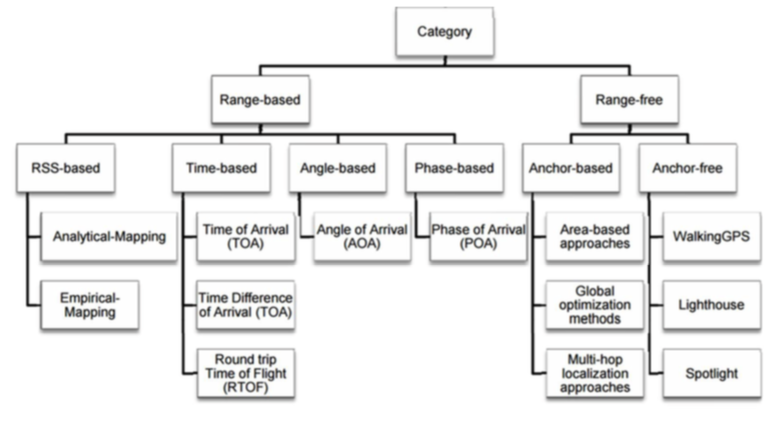
\includegraphics[width=6.26772in,height=3.41667in]{image8b.png}}
{Categorie di algoritmi}}
\label{categorie-di-algoritmi}

\begin{itemize}
\item
  \begin{quote}
  \textbf{Range based}: inferiscono la posizione tenendo conto della
  distanza tra i vari nodi
  \end{quote}

  \begin{itemize}
  \item
    \begin{quote}
    \textbf{RSS-Based} (\textbf{Received Signal Strength}) la distanza
    dai nodi viene calcolata tenendo conto dell'intensità del segnale
    ricevuto, tenendo conto della perdita dovuta all'ambiente
    circostante.\(RSS(d)\  = \ P_{t}\  \times \text{K\ } \times (\frac{d_{0}}{d})^{n}\)
    dove \(P_{t}\) è a potenza di trasmissione, \emph{K} è una costante,
    \(d_{0}\)è la perdita di potenza (\textbf{path loss)} fino al punto
    di riferimento e \(n\) dipende dall'ambiente. Basando
    sull'\textbf{RSS} si può definire l'\textbf{Analytical Mapping
    Model}:
    \end{quote}
  \end{itemize}
\end{itemize}

\begin{quote}
\(RSS(d)\lbrack dB\rbrack\  = \ RSS(d_{0})\  - \ 10n\ \log(d/d_{0})\  + \ X_{\backslash sigma}\lbrack dB\rbrack\)dove
\(X_{\backslash sigma}\)è una variabile casuale gaussiana che
rappresenta la varianza. Sfortunatamente questo modello è inaffidabile
perché non sempre la gaussiana va bene. Nell'\textbf{Empirical Mapping}
viene prima misurata dal distanza RSS con degli esperiementi, dopodiché
vengono definite delle regioni in cui inserire degli access point che
trasmettono un segnale ad intensità regolare. Il nodo quindi rileva
questi segnali e utilizza un classificatore per capire in quale delle
regioni si trova, tenendo conto delle misurazioni precedentemente
effettuate. Questo secondo modello è molto più affidabile ma richiede
una profilazione dell'ambiente (che deve essere statico) ed elevate
capacità di calcolo, pertanto è poco scalabile.
\end{quote}

\begin{itemize}
\item
  \begin{quote}
  \textbf{Time Based}: la stima della posizione viene effettuata tenendo
  conto del tempo di propagazione del segnale radio.
  \end{quote}

  \begin{itemize}
  \item
    \begin{quote}
    \textbf{Time of Arrival (ToA):} assumendo che le comunicazioni dei
    nodi siano sincronizzate, utilizza il tempo di propagazione di un
    messaggio per approssimare la distanza. Funziona bene per le lunghe
    distanze (GPS) ma è necessaria la sincronizzazione dei nodi.
    All'aumentare della frequenza del segnale radio l'accuratezza
    migliora.
    \end{quote}
  \item
    \begin{quote}
    \textbf{Round-Trip Time of Flight (RTOF)}: approssima la distanza
    tenendo conto del tempo impiegato da un messaggio per ritornare. Non
    richiede la sincronizzazione ma è più soggetta ad errori dovuti al
    rumore del segnale.
    \end{quote}
  \item
    \begin{quote}
    \textbf{Time Difference of Arrival (TDoA):} il nodo che deve
    inferire la posizione riceve due segnali a frequenze diverse,
    tipicamente uno Radio e uno Ultrasuono e calcola la distanza in base
    alla differenza d'arrivo dei due segnali, prendendo come riferimento
    il più veloce (\textbf{Single Receiver}). Così facendo non serve la
    sincronizzazione dei nodi e il consumo di energia è ridotto. In
    alternativa è possibile utilizzare due ricevitori posti a distanza
    nota ed approssimare la distanza dalla sorgente utilizzando la
    differenza nel tempo di ricezione del segnale da parte dei due
    ricevitori (\textbf{Multiple Receiver})
    \end{quote}
  \end{itemize}
\item
  \begin{quote}
  \textbf{Angle of Arrival}: utilizza l'angolo di arrivo del segnale per
  capire in che direzione si trova il nodo sconosciuto in base
  all'ancora che ha ricevuto il segnale. Se è disponibile l'informazione
  riguardo l'orientamente delle varie ancore bastano solo due nodi
  ancora per inferire la posizione, altrimenti ne sono necessari tre.
  Per determinare l'angolo di arrivo di un segnale si può utilizzare
  un'antenna rotante (hardware costoso) oppure un array di antenne poste
  a distanza fissa tra loro in modo da determinare l'angolo in base a
  come queste ricevono il segnale.
  \end{quote}
\end{itemize}

\begin{itemize}
\item
  \begin{quote}
  \textbf{Range Free:} la posizione viene inferita tenendo conto della
  prossimità rispetto ad alcuni target.
  \end{quote}

  \begin{itemize}
  \item
    \begin{quote}
    \textbf{Anchor based}: vengono predisposti dei nodi ancora in
    posizioni fisse e note a priori
    \end{quote}

    \begin{itemize}
    \item
      \begin{quote}
      \textbf{Area based approach}: la posizione viene calcolata come il
      \textbf{centroide} del poligono determinato da tutte le ancore
      alle quali il nodo è connesso. In alternativa si può suddividere
      lo spazio in triangoli e via via restringere l'area del triangolo
      in base alle ancore connesse.
      \end{quote}
    \item
      \begin{quote}
      \textbf{Multihop localization approach}: non sempre si hanno a
      disposizione abbastanza ancore. Con questo approccio ogni ancora
      invia una beacon con la sua posizione e con un
      \textbf{hop-counter}, quando le ancore ricevono uno di questi
      messaggi incrementano l'hop counter e lo rimandano alle altre
      ancore a loro connesse. Quando un nodo sconosciuto si connette ad
      un'ancora, questo riceve anche gli altri messaggi con la posizione
      della altre ancore fuori range e sfrutta queste informazioni per
      provare a determinare la sua posizione (\textbf{DV-Hop}). In base
      alla distribuzione delle ancore può essere necessaria una
      correzione più o meno aggressiva.
      \end{quote}
    \end{itemize}
  \item
    \begin{quote}
    \textbf{Anchor Free:} metodi guidati agli eventi che sfruttano le
    informazioni temporali e spaziali per inferire la posizione, con
    segnali di vario genere. Funziona sotto l'assunzione che certi
    eventi possono essere generati in un preciso istante e in una
    precisa posizione.
    \end{quote}

    \begin{itemize}
    \item
      \begin{quote}
      \textbf{Walking GPS:} c'è un nodo dotato di GPS che si muove e fa
      il broadcast della sua posizione.
      \end{quote}
    \item
      \begin{quote}
      \textbf{Lighthouse}: c'è un ancora che ruota a velocità costante
      ed emette un segnale luce.
      \end{quote}
    \end{itemize}
  \end{itemize}
\end{itemize}

\subsection{Tecniche di
geo-localizzazione}\label{tecniche-di-geo-localizzazione}

ovvero come trovare la posizione di un nodo sapendo la distanza o
l'angolazione del segnale.

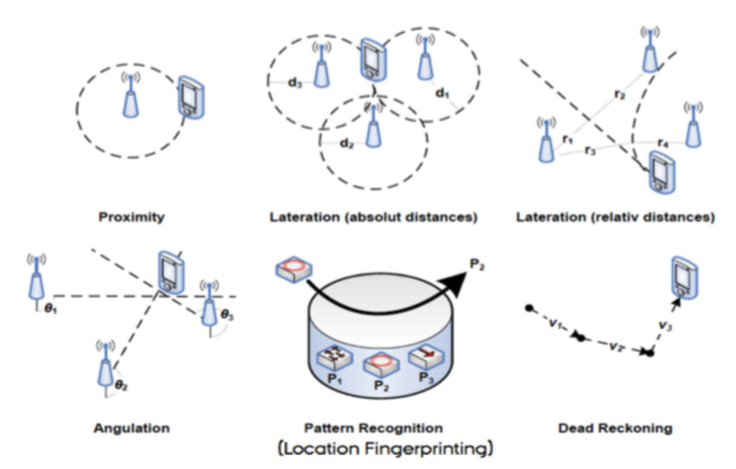
\includegraphics[width=6.26772in,height=4.00000in]{image6b.png}

\begin{itemize}
\item
  \begin{quote}
  \textbf{Lateration - Trilateration:} usa la distanza dalle ancore per
  stabilire la posizione del nodo. In assenza di rumore si tratta di
  risolvere un sistema lineare (intersezione di 3 o più cerchi)
  \end{quote}

  \begin{itemize}
  \item
    \begin{quote}
    \textbf{Bound-box}: versione meno accurata ma più efficiente che
    anziché calcolare la posizione precisa con i cerchi, utilizza i dei
    rettangoli per stimare una possibile \textbf{box} in cui si trova il
    nodo.
    \end{quote}
  \item
    \begin{quote}
    \textbf{Triangolazione (Triangulation)}: utilizza l'angolo di
    ricezione del segnale (\textbf{AoA approach}) per determinare la
    posizione.
    \end{quote}
  \item
    \begin{quote}
    \textbf{Multilateration}: utilizza delle misurazioni \textbf{TDoA}
    provenienti da vari nodi ancora.
    \end{quote}
  \item
    \begin{quote}
    \textbf{Closest Neighbor:} calcola la posizione tenendo conto delle
    ancore a cui è possibile connettersi.
    \end{quote}
  \end{itemize}
\end{itemize}

\subsection{Sistemi di localizzazione}\label{sistemi-di-localizzazione}

\begin{itemize}
\item
  \begin{quote}
  \textbf{Active badge:} un badge emette un segnale IR ad intervalli
  regolari che viene rilevato da dei sensori posti nell'edificio. La
  posizione è stimata in base al sensore che riceve il segnale.
  \end{quote}
\item
  \begin{quote}
  \textbf{Active Bat:} il personale è dotato di un trasmettitore ad
  ultrasuoni e nell'edificio sono posti dei ricevitori. La posizione
  viene calcolata in base all'intensità del segnale ricevuto mediante
  trilaterazione.
  \end{quote}
\item
  \begin{quote}
  \textbf{Ubisense}: utilizza \textbf{TDoA} e \textbf{AoA} in modo
  simile ad Active Bat.
  \end{quote}
\item
  \begin{quote}
  \textbf{Cricket}: version opposta di Active Bat, la componente attiva
  è nell'infrastruttura e il ricevitore è indossato dalla persona.
  \end{quote}
\item
  \begin{quote}
  \textbf{RADAR/PlaceLab}: utilizza le radio frequenze
  dell'infrastruttura Wi-Fi per stimare la posizione in base ad un
  \textbf{RSS} mappato, ovvero assumendo di conoscere la struttura
  dell'edificio.
  \end{quote}
\end{itemize}

\section{Mobile Sensing}\label{mobile-sensing}

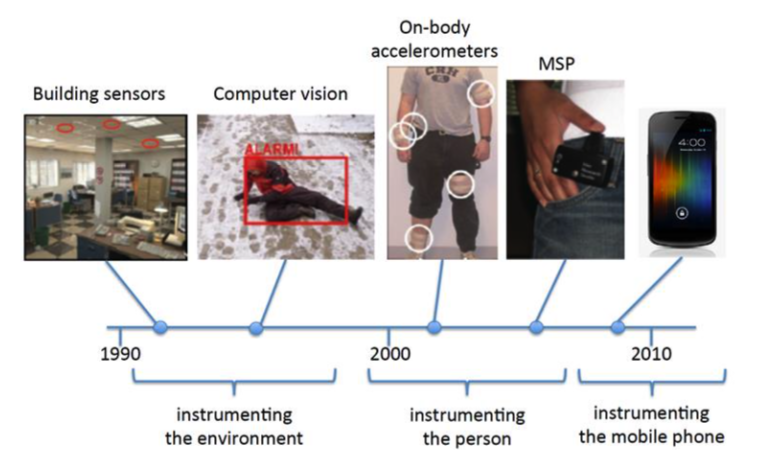
\includegraphics[width=6.26772in,height=3.86111in]{image4b.png}

Al giorno d'oggi la maggior parte dei telefoni è dotata di sensori
quali: accelerometro, giroscopio e microfono, che però sono stati
inseriti per implementare determinate funzionalità e non per recuperare
informazioni sull'ambiente circostante.

Solo ultimamente vengono forniti degli SDK per accedere ai dati
rilevati.

\begin{itemize}
\item
  \begin{quote}
  \textbf{Sensors Networks:} componenti ottimizzati per estrarre
  informazioni sull'ambiente circostante, molto precisi ed efficienti,
  ma molto costosi da predisporre/mantenere.
  \end{quote}
\item
  \begin{quote}
  \textbf{Phone sensing}: sensori presenti nei telefoni, utili per
  rilevare le attività dell'utente ma poco precisi. Costi di
  manutenzione praticamente nulli, ammesso che l'utente installi l'app
  sul telefono.
  \end{quote}
\end{itemize}

\subsection{Applicazione del
mobile-sensing}\label{applicazione-del-mobile-sensing}

\begin{itemize}
\item
  \begin{quote}
  \textbf{Individuale:} fitness/comportamento dell'utente.
  \end{quote}

  \begin{itemize}
  \item
    \begin{quote}
    Attività fisica: camminata, corsa, scale. Rilevata mediante
    accelerometro, giroscopio e bussola.
    \end{quote}
  \end{itemize}
\item
  \begin{quote}
  \textbf{Group/community:} attività di gruppo oppure obiettivi comuni,
  come la sorveglianza di quartiere.
  \end{quote}
\item
  \begin{quote}
  \textbf{Urban scale}: aggregazione di dati per fornire informazioni
  utili alla comunità, tipo Waze per il traffico.
  \end{quote}

  \begin{itemize}
  \item
    \begin{quote}
    Informazioni sui trasporti: biciclette e mezzi pubblici. Rilevate
    con accelerometro, GPS e Wi-Fi, per raccogliere dati ed agevolare il
    trasporto delle persone
    \end{quote}
  \end{itemize}
\end{itemize}

\subsection{Design di un'applicazione}\label{design-di-unapplicazione}

\begin{enumerate}
\def\labelenumi{\arabic{enumi}.}
\item
  \begin{quote}
  \textbf{Raccolta di dati grezzi:} vengono utilizzati i sensori per
  raccogliere i dati
  \end{quote}
\item
  \begin{quote}
  \textbf{Inferenza dell'attività in corso:} machine learning per dare
  un significato ai dati
  \end{quote}
\item
  \begin{quote}
  \textbf{Generazione di dati di alto livello:} aggregazione di
  statistiche
  \end{quote}
\end{enumerate}

Bisogna tenere a mente che l'utilizzo dei sensori richiede molte
risorse: batteria, CPU, memoria e archiviazione. Serve quindi un
bilanciamento nell'utilizzo dei sensori e nella precisione richiesta per
evitare di consumare troppe risorse.

Modalità di rilevamento:

\begin{itemize}
\item
  \begin{quote}
  \textbf{Continuous:} viene effettuato un campionamento continuo dei
  dati forniti dal sensore e man mano che arrivano nuovi dati viene
  fatta inferenza. Si ottiene così un elevata precisione ma con elevati
  consumi.
  \end{quote}
\item
  \begin{quote}
  \textbf{Duty cycling}: il campionamento viene fatto ad intervalli
  regolari di una certa durata. Più efficiente in termini di risorse ma
  meno preciso. C'è il rischio che alcuni eventi vengano persi.
  \end{quote}
\item
  \begin{quote}
  \textbf{Adaptive Duty Cycling:} come il Duty cycling solo che se viene
  rilevato un evento, viene aumentata la frequenza di campionamento per
  aumentare la precisione. Se non vengono rilevati eventi la frequenza
  di campionamento decresce. Tipicamente con andamento lineare o
  esponenziale, in base alla tipologia di applicazione. Serve pertanto
  una buona conoscenza del dominio.
  \end{quote}
\end{itemize}

L'inferenza viene effettuata tipicamente con una pipeline di machine
learning che prima ripulisce i dati e poi li classifica. La prima parte
di pulizia può sfruttare informazioni pre-calcolate durante una fase di
training. La classificazione viene invece effettuata tipicamente in modo
probabilistico (Bayes) o con alberi di classificazione.

Per ridurre l'impatto energetico dell'inferenza questa può essere
spostata su un computer remoto, aggiungendo però i problemi e i costi
legati alla comunicazione tra il dispositivo e il server. La pipeline
può essere anche ibrida, con la feature extraction/pulizia dei dati
fatta dal dispositivo e con la classificazione effettuata in remoto.
